%----------------------------------------------------------------------------
%	PACKAGES AND OTHER DOCUMENT CONFIGURATIONS
%----------------------------------------------------------------------------

\documentclass[idxtotoc,hyperref,openany]{labbook}

\usepackage[ 
  backref=page,
  pdfpagelabels=true,
  plainpages=false,
  colorlinks=true,
  bookmarks=true,
  pdfview=FitB]{hyperref}
  
\usepackage{booktabs}
\usepackage{float}
\usepackage{graphicx}
\usepackage{lipsum}
\usepackage{siunitx}

\graphicspath{Figures/}

\newcommand{\HRule}{\rule{\linewidth}{0.5mm}}
\setlength\parindent{0pt}
\setlength{\parskip}{\baselineskip}

%----------------------------------------------------------------------------
%	DEFINITION OF EXPERIMENTS
%----------------------------------------------------------------------------

\newexperiment{PPDr}{PPD Repair After PaCE-2022}
\newexperiment{FibrePull}{Manufacturing Glass Fibres}
\newexperiment{MeetPID}{PID Weekly Meeting}
\newexperiment{MAZ04}{Construction of UCASS Batch MAZ04}
\newexperiment{MPICCE}{Mixed-Phase and Ice Cloud Characterisation Experiment}

%----------------------------------------------------------------------------

\begin{document}

%----------------------------------------------------------------------------
%	TITLE PAGE
%----------------------------------------------------------------------------

\frontmatter % Use Roman numerals for page numbers
\title{
\begin{center}
\HRule \\[0.4cm]
{\Huge \bfseries Laboratory Journal}\\[0.4cm]
\HRule \\[1.5cm]
\end{center}
}
\author{\Huge Jessica Girdwood \\ \\ \LARGE jessgirdwood@protonmail.com \\[2cm]}
\date{Beginning 20\textsuperscript{th} March 2023}
\maketitle

\tableofcontents

\mainmatter

%----------------------------------------------------------------------------
%	LAB BOOK CONTENTS
%----------------------------------------------------------------------------

\labday{20 March 2023}

\experiment{PPDr}

PPD is no longer functional after returning from a campaign in northern Finland. There are no useful images on the screen. When the trigger threshold is lowered to 10, and the trigger PMT voltage is raised above 20, there are noise triggers.

PPD was removed from its pelicase, removing and breaking the seal of the 4 bolts. The inlet heaters were disconnected, and the pump was removed. The arduino was reprogrammed to not trigger the relays. PPD was suspended above  the pelicase on two poles. The grounding point was replaced and connected to the mains socket, the mains cable was also replaced with an English plug.

\labday{21 March 2023}

\experiment{PPDr}

When the output of the trigger PMT was observed with a scope, the signal looked extremely noisy, and repeated at around \SI{5.6}{\kilo\hertz}. Figure \ref{fig:PPDScopeNoise} shows this. I was unable to determine as to whether this was the laser or the PMT, however the laser was visibly damaged so this was the suspected cause at this stage.

\begin{figure}[H]
\begin{center}
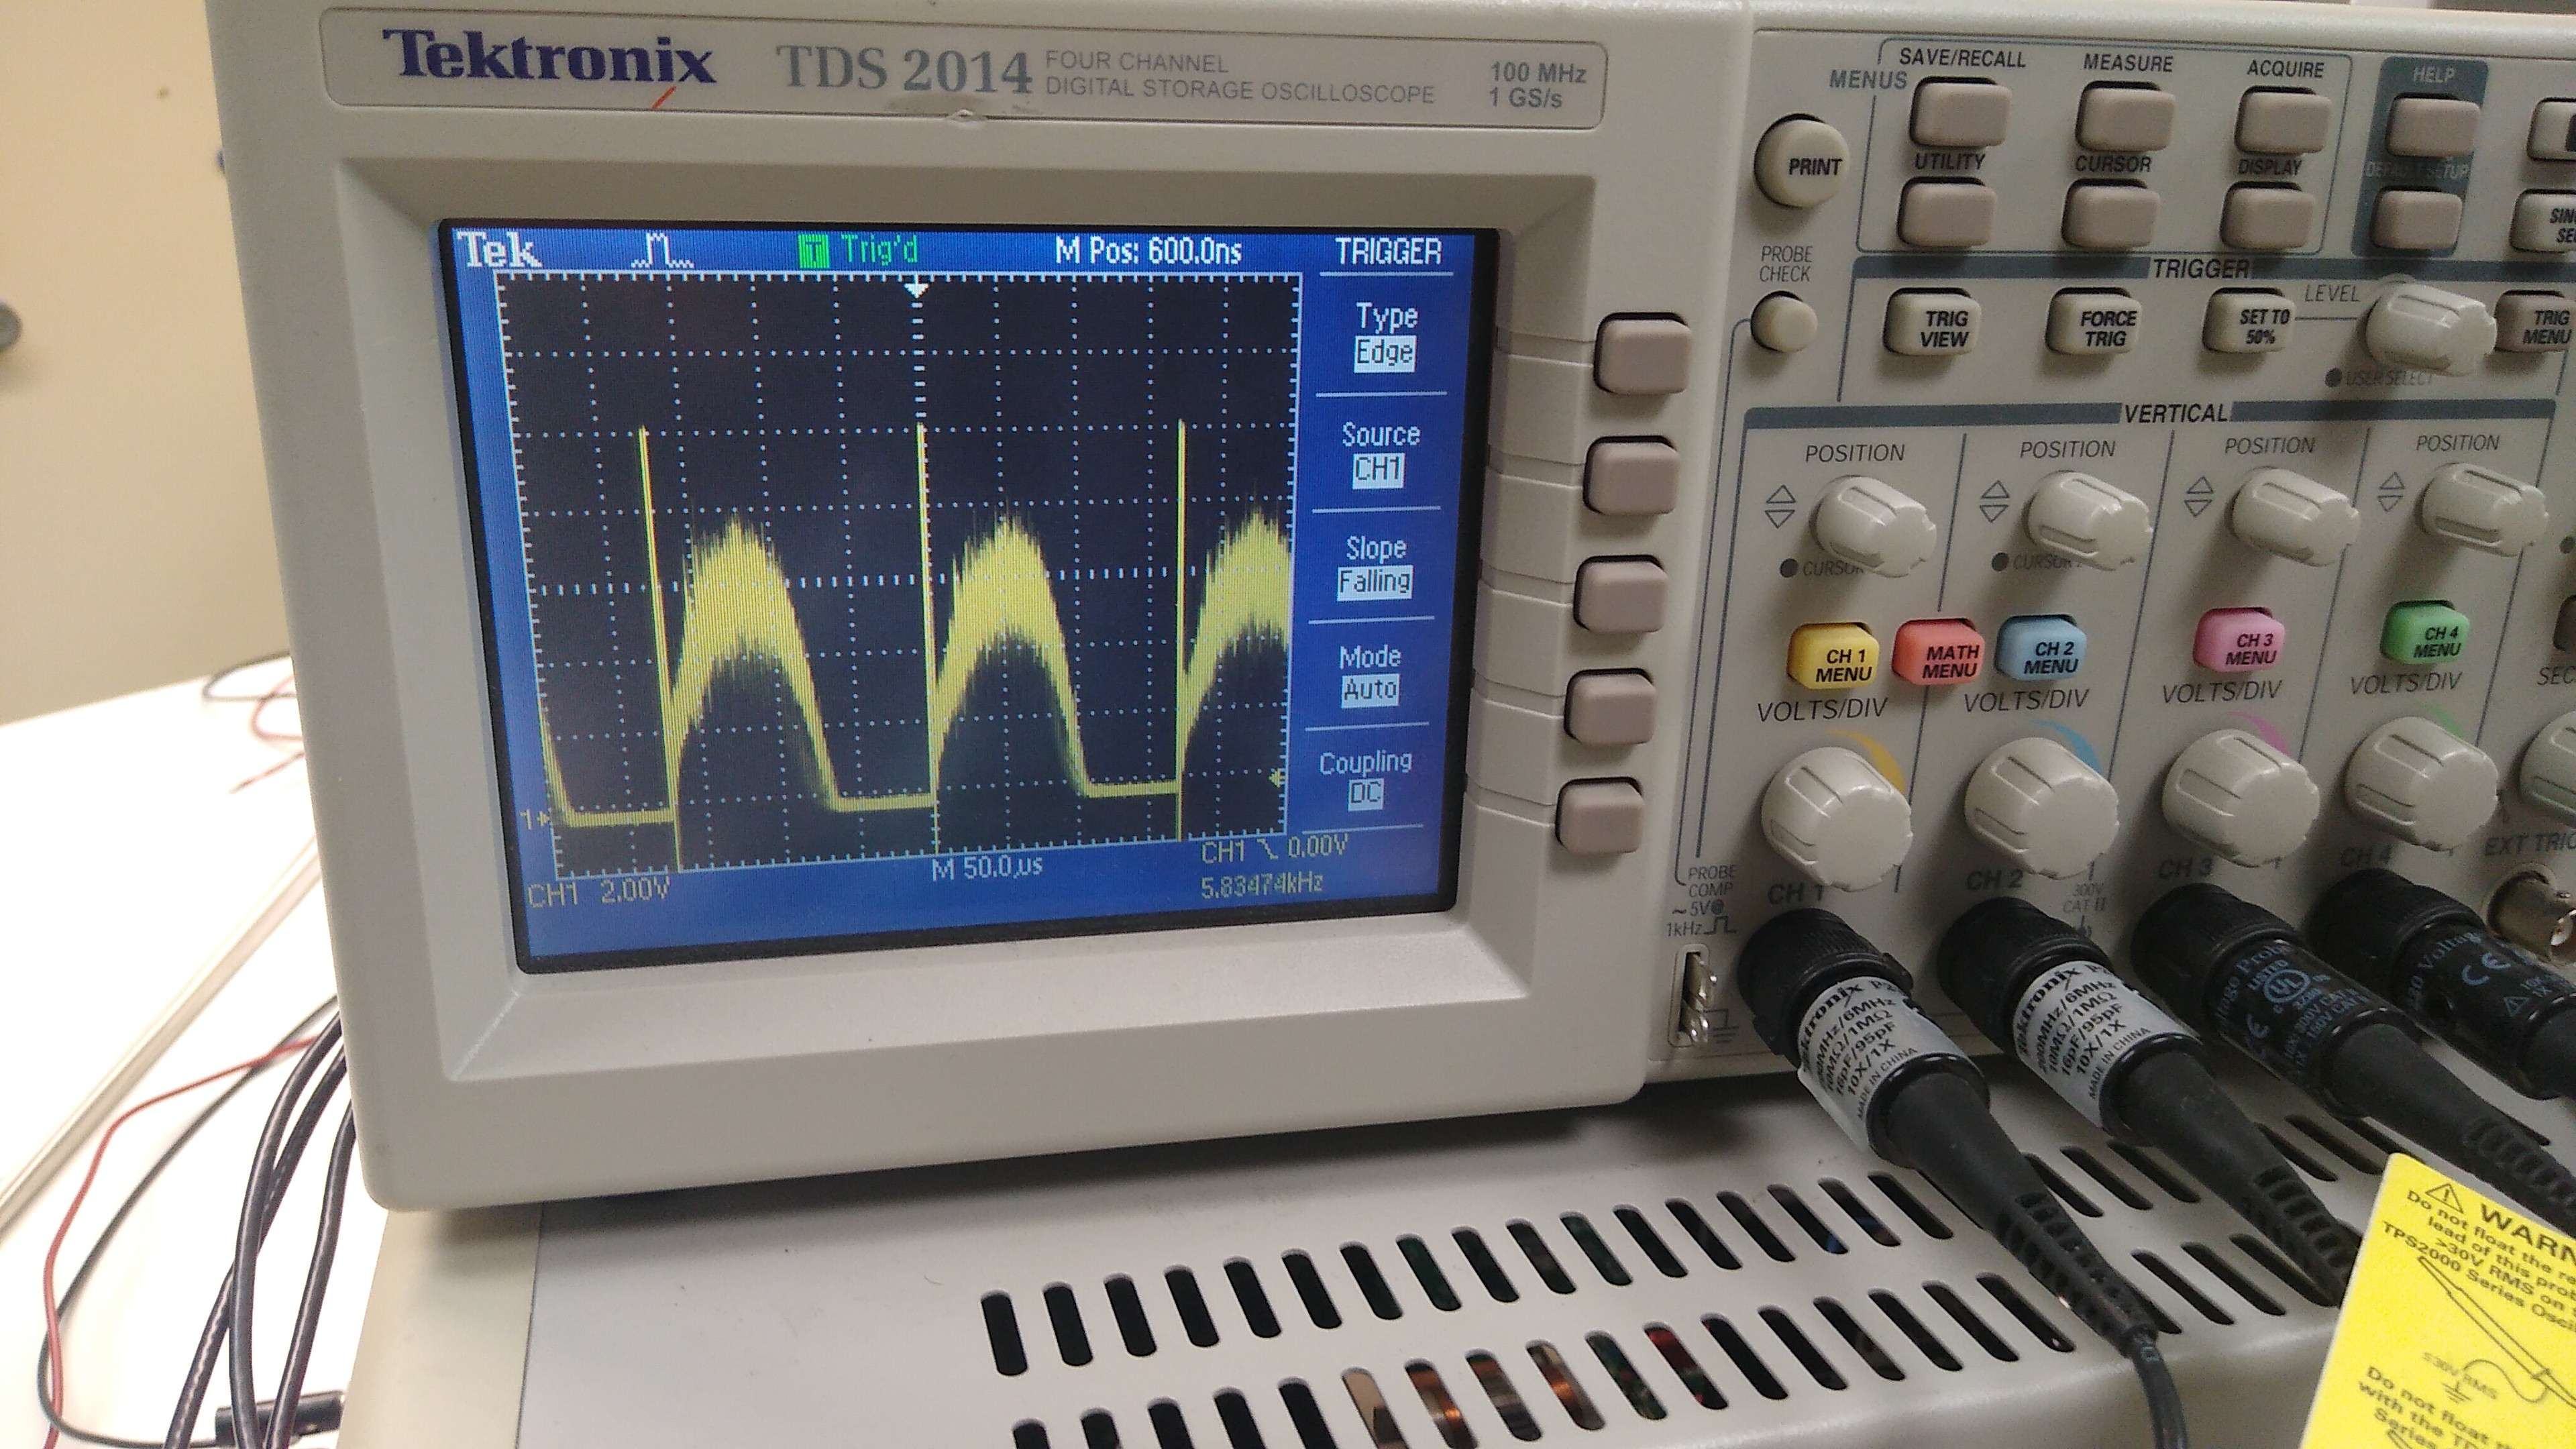
\includegraphics[width=0.5\linewidth]{Figures/PPDScopeNoise}
\end{center}
\caption{Noise after campaign with old laser.}
\label{fig:PPDScopeNoise}
\end{figure}

When an object was inserted into the optics chamber, the output resembled a square wave. This is shown in Fig. \ref{fig:PPDScatterOutput}.

\begin{figure}[H]
\begin{center}
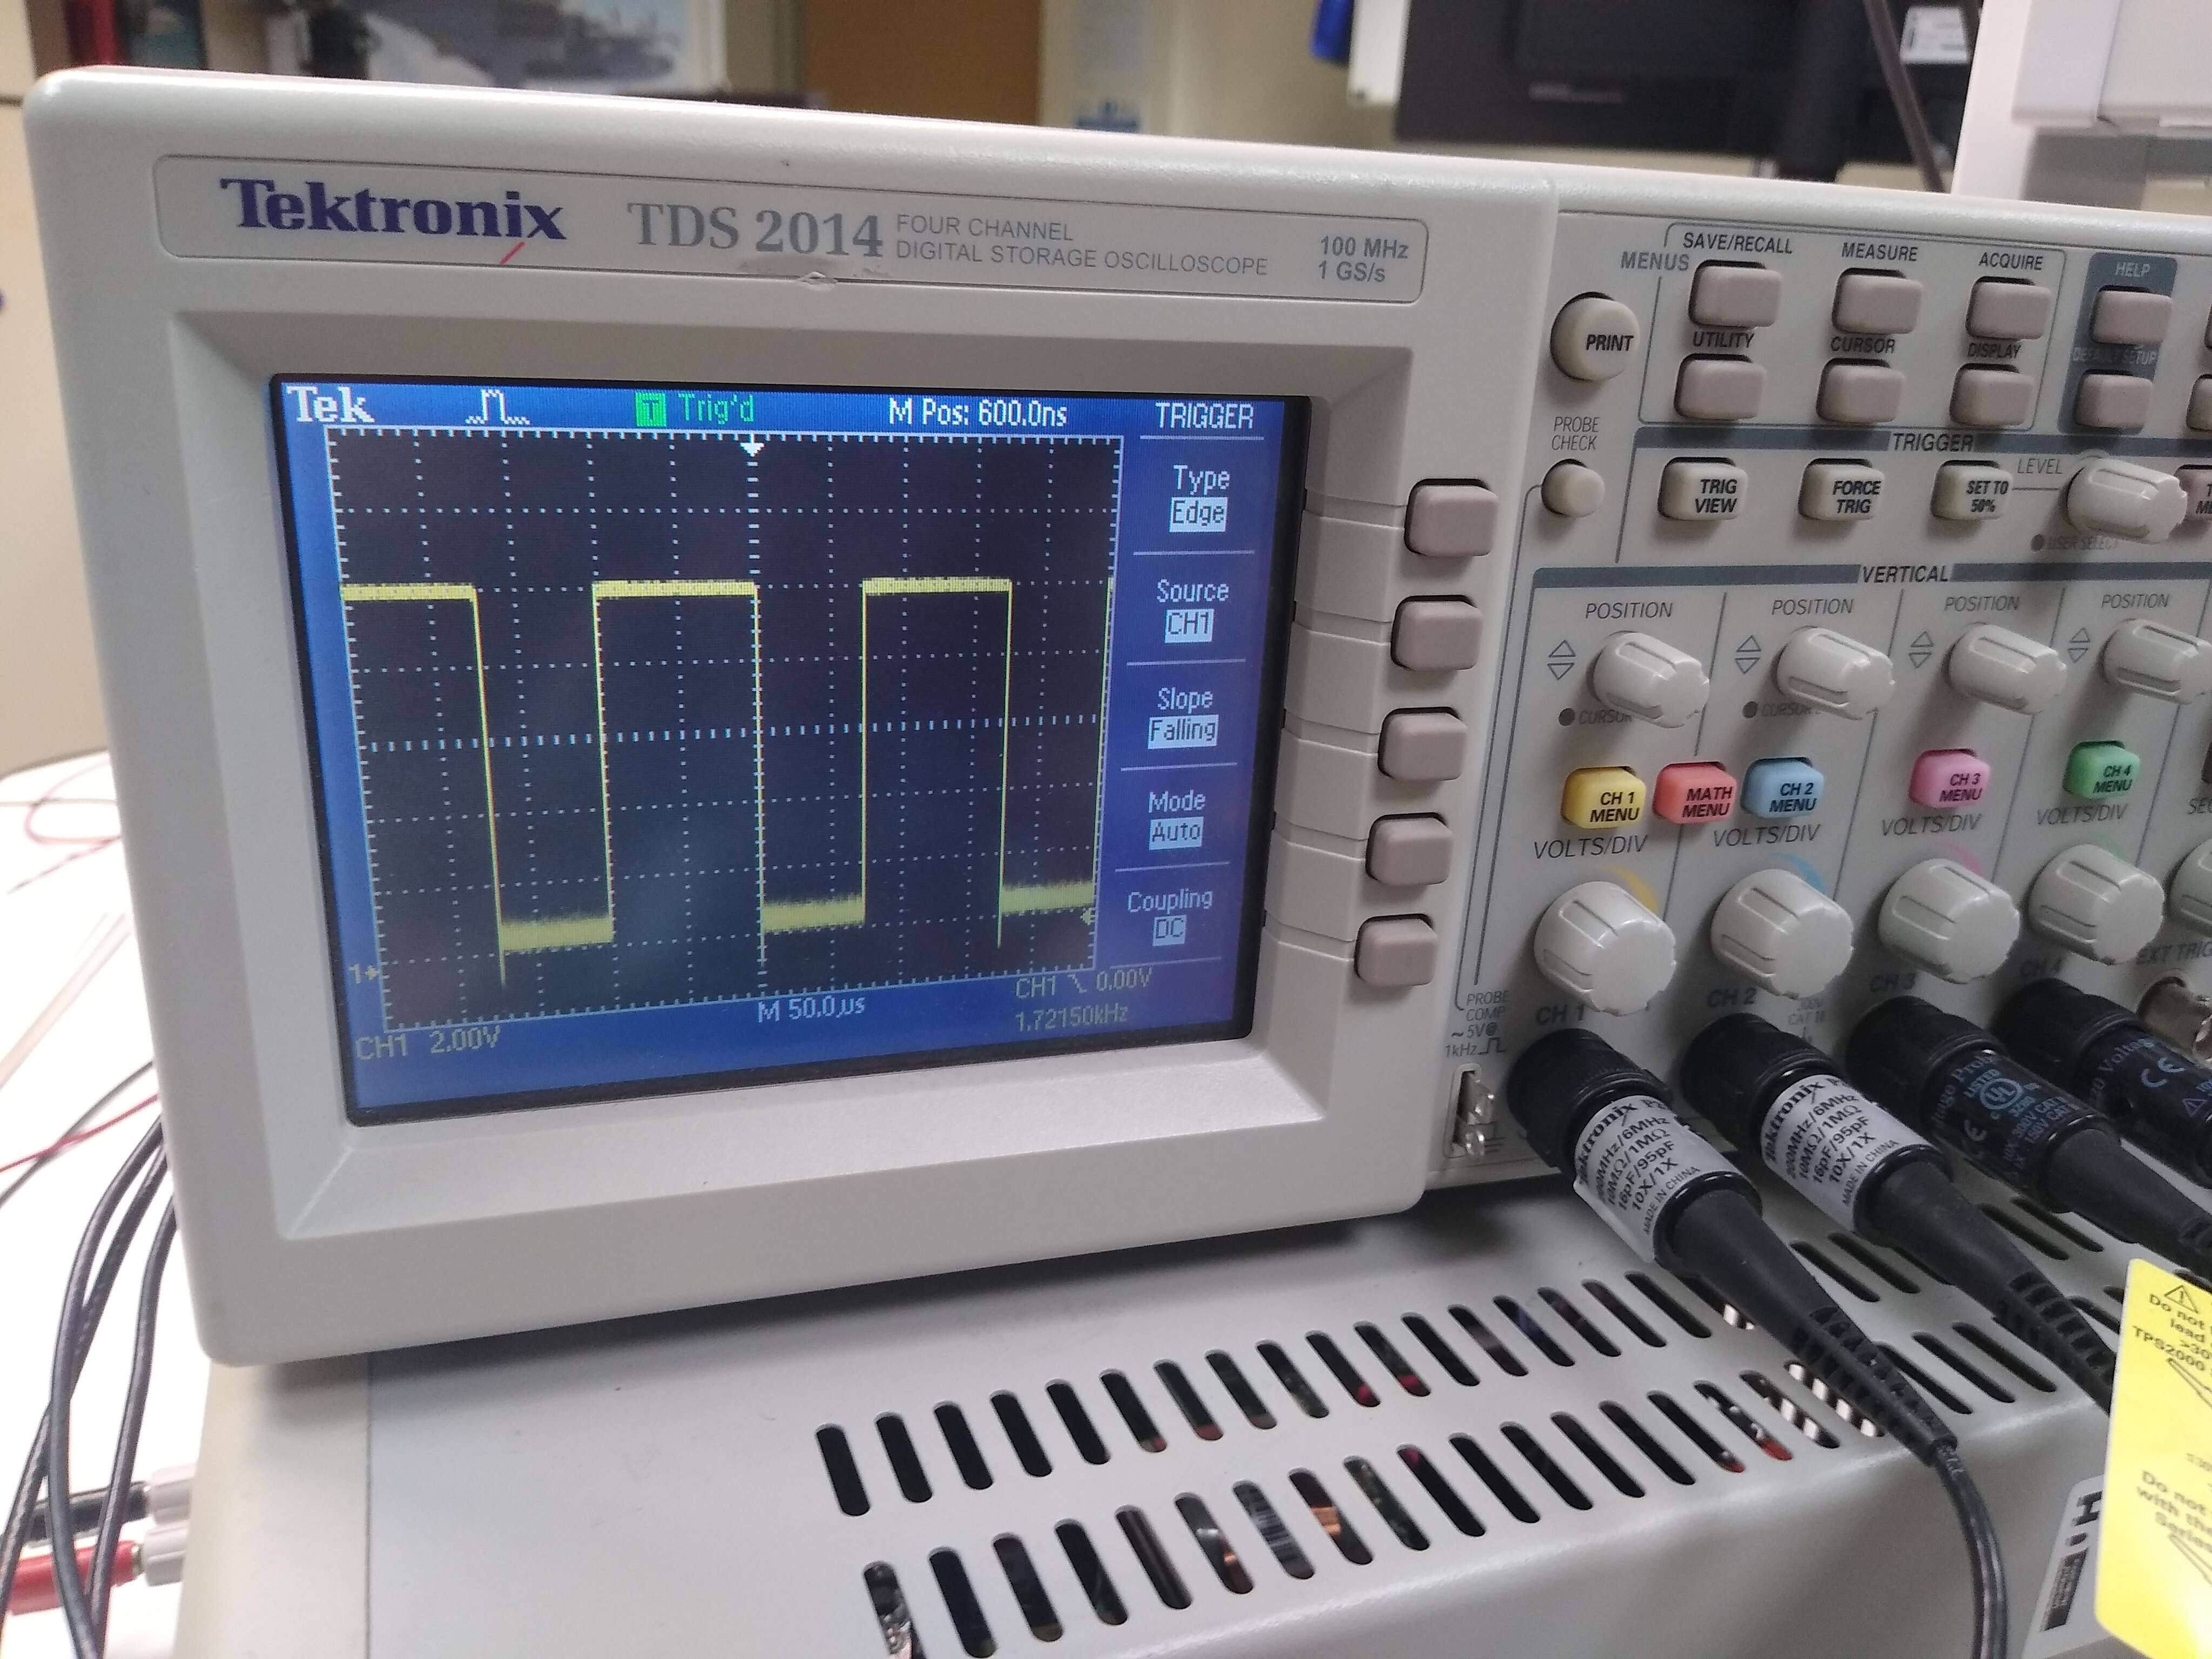
\includegraphics[width=0.5\linewidth]{Figures/PPDScatterOutput}
\end{center}
\caption{Noise after campaign with old laser and object in beam.}
\label{fig:PPDScatterOutput}
\end{figure}

The beam was also visibly dimmer, which would explain the lower image intensity. A pulse generator was configured to trigger the camera with a simulated 5 particles per second, each with a \SI{10}{\micro\second} pulse width. The camera triggering was unreliable, oftentimes exhibiting the characteristics of a "busy port".

It was decided that a new laser was the preferable option. A replacement CrystaLaser \SI{532}{\nano\metre} at \SI{150}{\milli\watt} was located.

\labday{29 March 2023}

\experiment{PPDr}

The new laser needed to be aligned since it hit the beamstop in the incorrect place, and did not pass straight through the aperture in the chamber. It was determined at a first glance that the previous alignment system would be unsuitable fo use, since it was locked in place with cyano-threadlocker. The two axes of motion couold be acheived by moving the laser on the screws, and placing shims beneath the laser to raise or lower it in one place.

It was found that the four mounting screws did not leave enough motion to rotate the laser laterally into the correct position. Two screws were removed, and the correct displacement could therefore be acheived. However, at this point, the images provided by PPD were not bright enough, and the laser was still visibly dark. An alignment tool was constructed from 3d printed PLA and a \SI{55}{\micro\metre} fibre, which could be screwed into the scattering chamber and intersect the beam. Figure \ref{fig:PPDFibreScatter} shows the scattering off the fibre, with the camera being triggered by a pulse generator, and the trigger PMT disconnected. The shape of the output seems reasonable, but the intensity of the image is very low, and the laser was visibly dim.

\begin{figure}[H]
\begin{center}
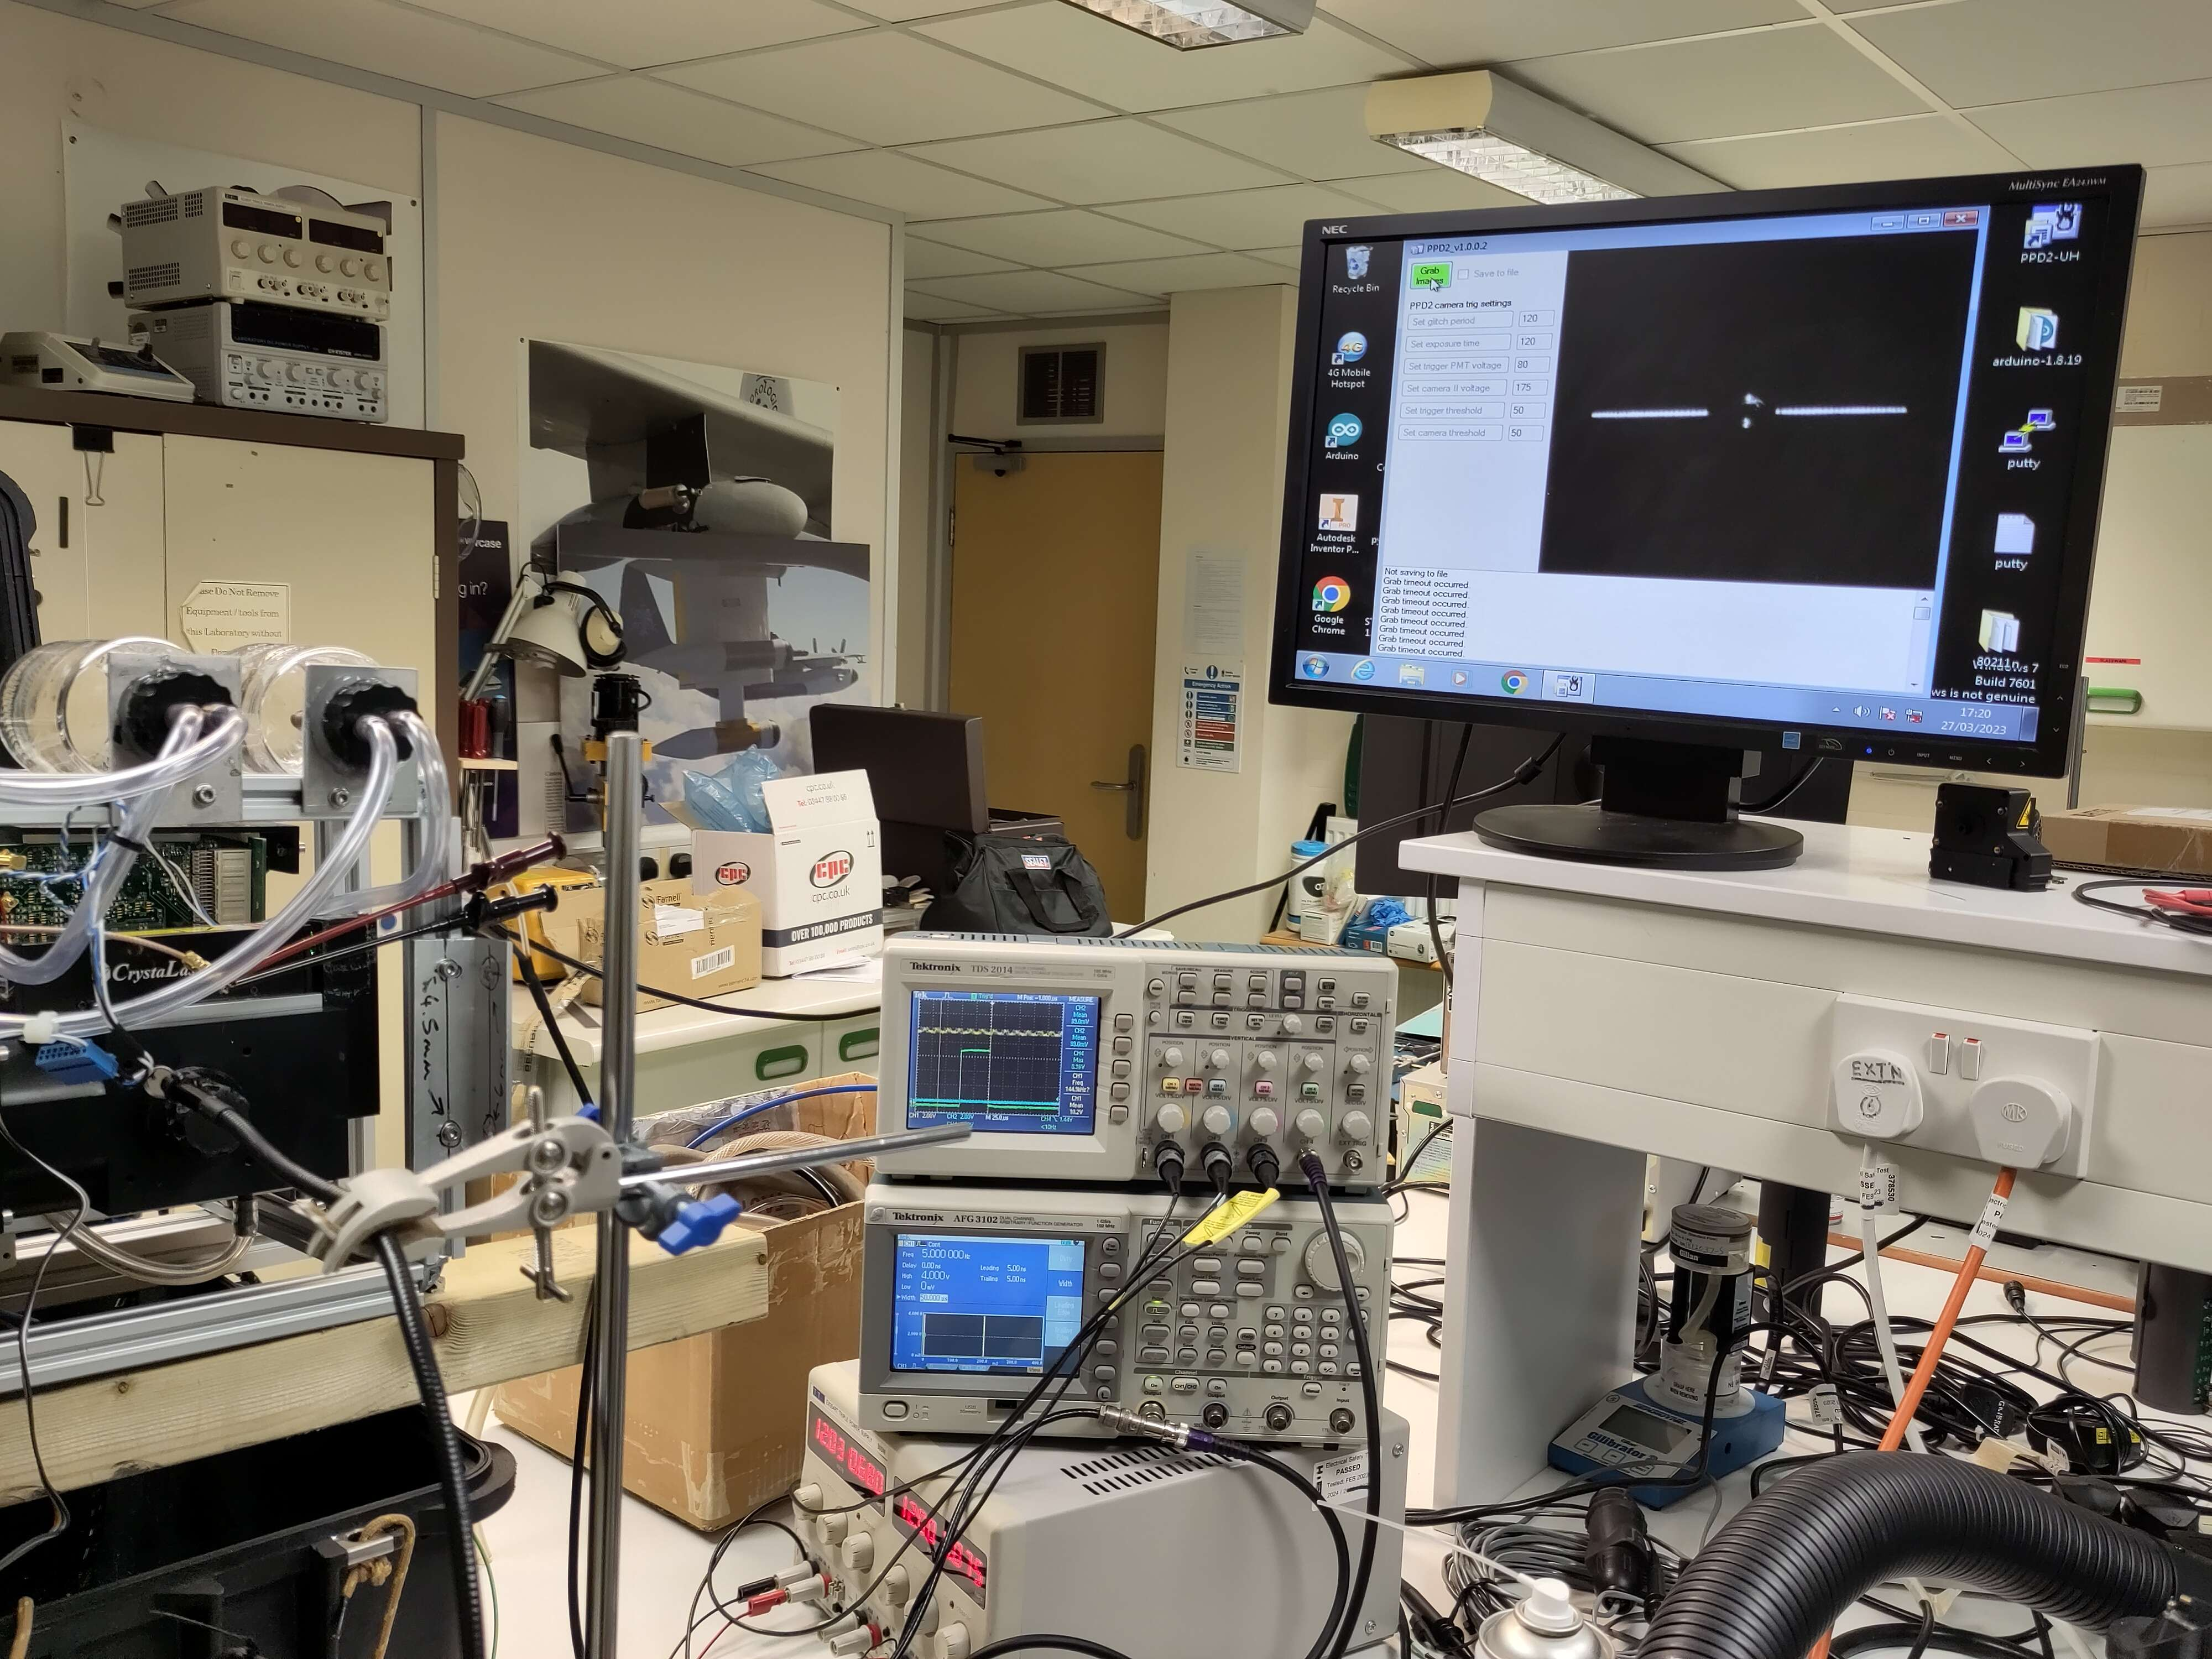
\includegraphics[width=0.5\linewidth]{Figures/PPDFibreScatter}
\end{center}
\caption{Scattering offf fibre tool.}
\label{fig:PPDFibreScatter}
\end{figure}

In order to observe the laser to further dianose issues, a beamview camera was used. The laser was reflected out of the optical block with a mirror, through an OD 2.0 neutral density filter, which lowered the output beam power to below \SI{1}{\milli\watt}, thus making it class 1. The beam appeared extremely low-quality, and looked more like diffraction off the aperture.

When the laser was tilted upwards, the beam quality improved. It was therefore determined that shims needed to be positioned beneath the front of the laser in order to acheive the desired alignment. Tilting of the laser adjusted the position of the beam relative to the aperture. It was determined through trail and improvement that two peices of paper or seven peices of foil were perfect, this is pictured in Fig. \ref{fig:PPDFoilLaser}

\begin{figure}[H]
\begin{center}
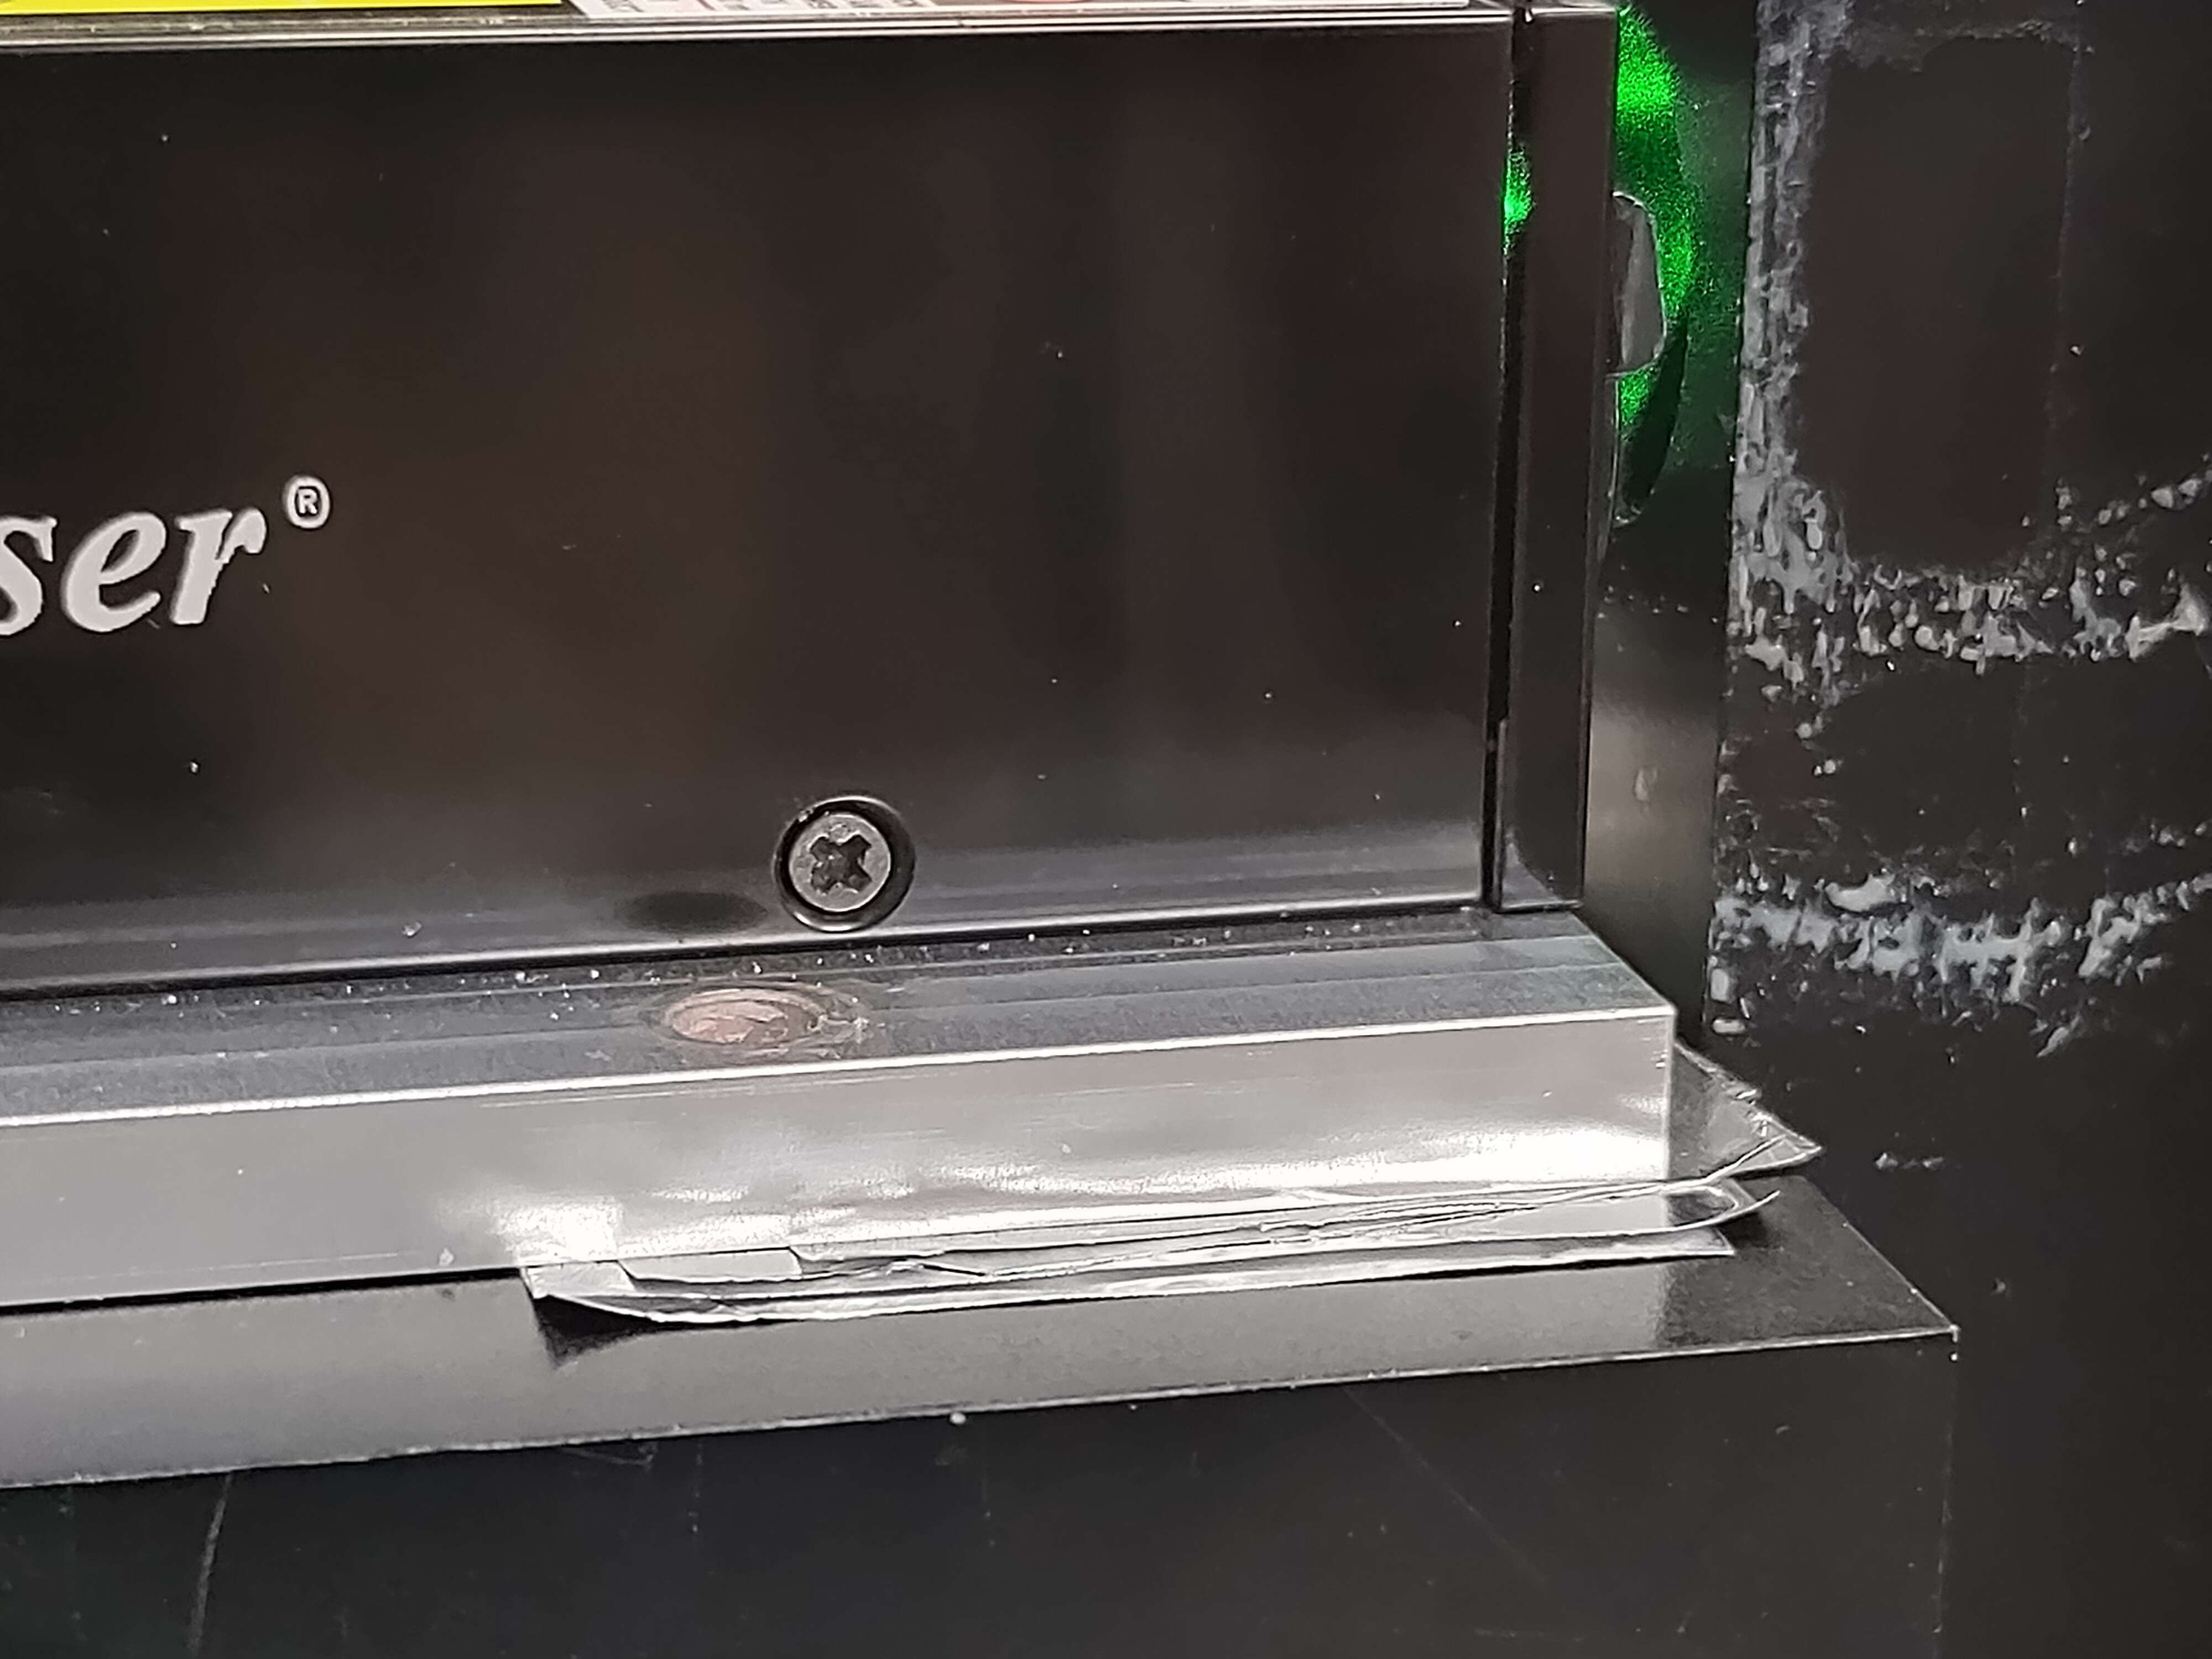
\includegraphics[width=0.5\linewidth]{Figures/PPDFoilLaser}
\end{center}
\caption{Image of foil beneath laser required for alignment.}
\label{fig:PPDFoilLaser}
\end{figure}

\labday{30 March 2023}

\experiment{PPDr}

The PPD was re-assembled for testing, the trigger PMT was re-connected. A new pump was fitted since the old one was broken by (suspected) water ingress. The flow of the pump was adjusted until \SI{6}{\litre\per\minute} was shown on the gilibrator flow-meter. Droplets were observed on the detector nicely :)

\begin{figure}[H]
\begin{center}
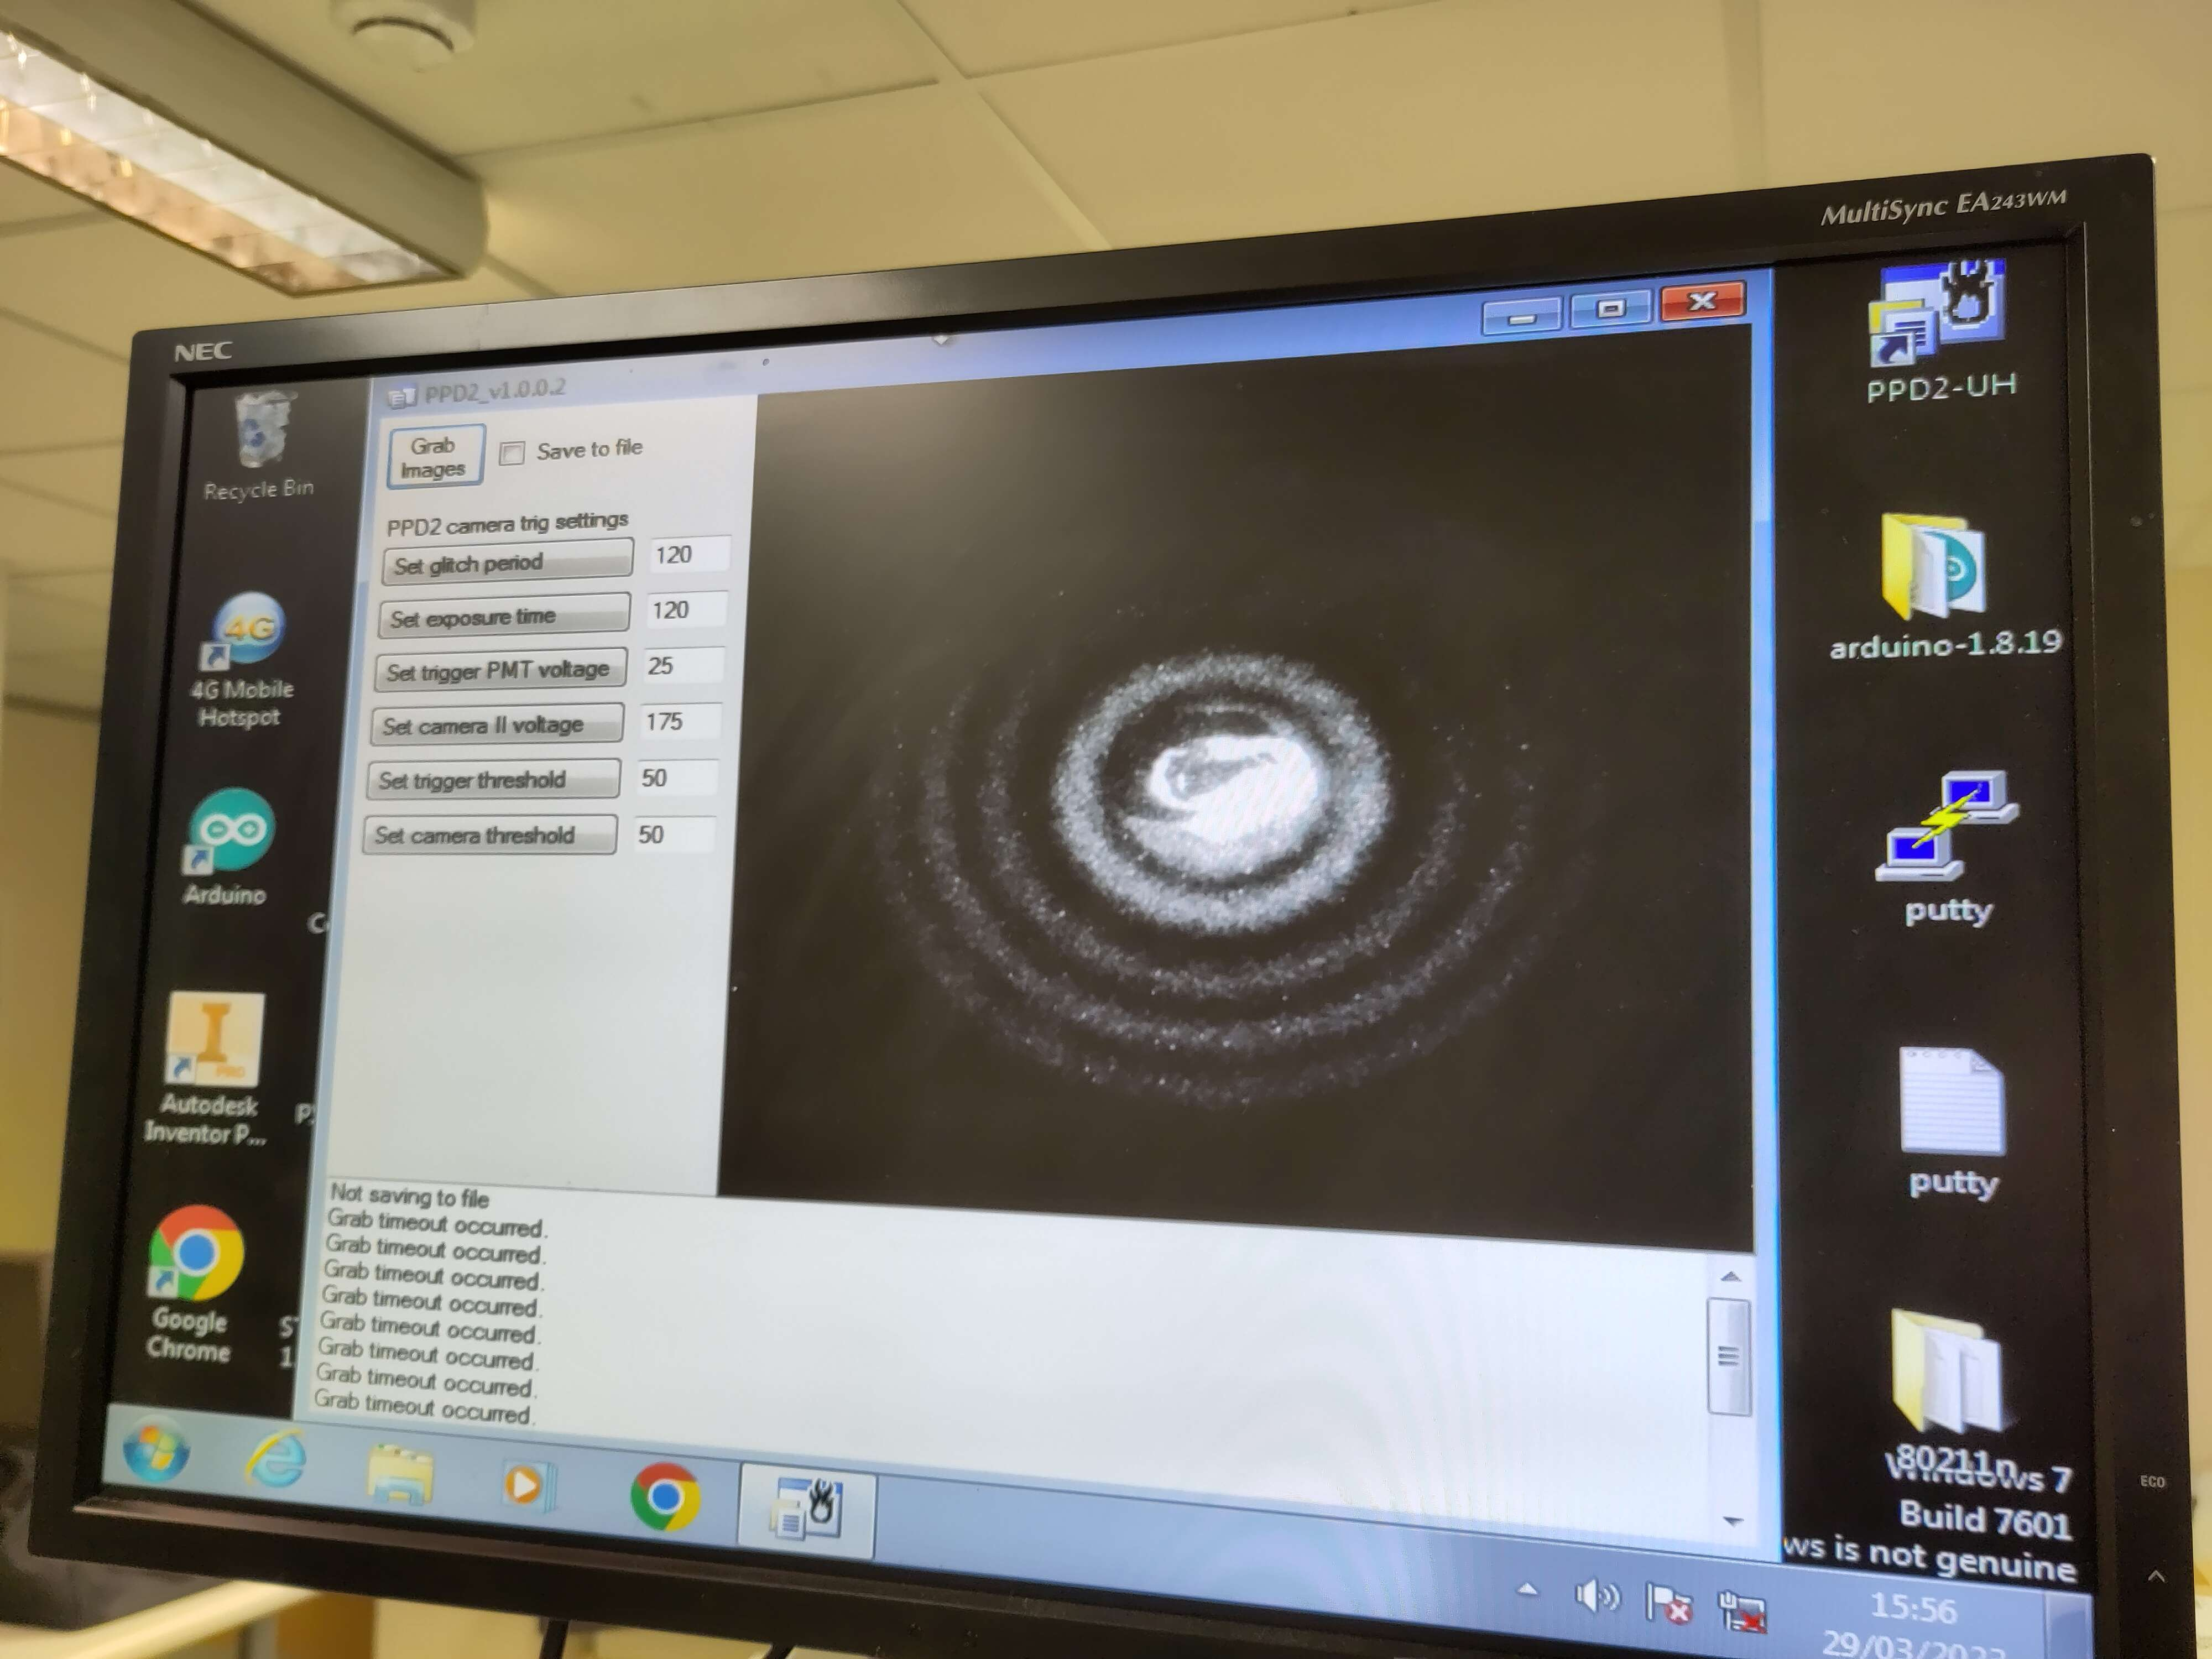
\includegraphics[width=0.5\linewidth]{Figures/PPDDropletImage}
\end{center}
\caption{Image of droplet scattering.}
\label{fig:PPDDropletImage}
\end{figure}

Ther eis still a huge problem with the computer images. There is a grab timeout which seems to randomly occur. Using a new computer with a firewire port which does not go through a PCI slot fixed the issue. It was determined that waiting for the latte-panda computer to arrive would be the preferable option for the new system. In addition, it was determined that transfering the PPD to a new case was the preferable option.

\labday{3 April 2023}

\experiment{FibrePull}

In order to achieve fibre calibrations, small fibres must be constructed. Bill Martin has lent us a pipette puller, which he has had some success with.

\experiment{MAZ04}

\begin{itemize}
\item 5 UCASS units from the batch do not work.
\item The diodes are attached firmly.
\item The laser power is reasonable.
\item The alignment is reasonable.
\item They all draw either too much or too little current.
\end{itemize}

In order to test the UCASS units, the fibre-LED setup was used with the outputs of the TIAs monitored.

\textbf{UCASS-AD-MAZ04-011:}

The unit was drawing too little current. The connections between boards were in the correct order, and there were no visible shorts. Wires were soldered onto the TIA outputs and to a grounding point (this will also be used for the fibre calibration at a later date). The scope output was positive-going when observed with a scope, however turned negative-going after wiggleing some wires around, when a fibre was inserted into the beam, the voltage dropped on both detectors, indicating the prsence of something in the beam. The outer detector was saturated, but the inner was not (potential bad alignment). There were still no counts on the software.

I attempted to reprogram the board with the 12id firmware. However, the unit stopped being able to read the infostring part-way through, and threw errors at me. After the laser is warmed up, the unit now draws the correct amount of current. The bootloader was re-programmed and the 13spi firmware was loaded onto the board. ExpBins were programmed, and the GSC was set to 1. The device still registered no counts or reject counts with the water spray. \textbf{This unit has been marked for realignment of elipsoidal mirror}.

\textbf{UCASS-AA-MAZ04-001:}

The unit was drawing too little current. Wired were soldered to the outputs of the TIAs (along with a grounding wire) and the output was measured when a fibre was inserted into the device. The fibre saturated both detectors, which indicates reasonable alignment. As with the previous unit, the current stealily rose as the laser warmed up.

\experiment{MeetPID}

\begin{itemize}
\item New laptops.
\item Warren has a flashing light on a uOPC.
\item Rob's update on fibre pulling. Currently the fibre is snapping before pulling.
\item Myriad can be used as a noun or an adjective.
\end{itemize}




\labday{4 April 2023}

\experiment{MAZ04}

\textbf{UCASS-AA-MAZ04-001 continued:}

It was decided, in order to rule out firmware or software issues, that the UCASS could be triggered using the fibre LED to view output counts. The laser turned itself off, but was reactivated when the unit was power-cycled. Blue-tac was positioned over the beamstop, the lights were switched off. The frequency of the pulse-generator was set to \SI{10}{\hertz} for 10 particles per second, the pulse width to \SI{10}{\micro\second}, and the ampitude to \SI{1}{\volt}---enough to activate the LED but not saturate the TIA. There were no couts observed, which indicates that the problem lies in the electronics as opposed to the alignment. This was conducive to the results of the fibre measurement. Inspection of the unit confirmed that one of the opamps responsible for DC-restoration was not attached properly, which was due to bad soldering. The chip was soldered on properly, and the other opamps were checked for defects (one other was found), I now believe this is what was wrong with 011 and will check the board again before removing the mirror. The unit now draws the correct amount of current. \textbf{Counts are now registered at \SI{1179}{ADC} for an input of \SI{900}{\milli\volt}}. The device now works properly with sample aerosol.

\textbf{UCASS-AD-MAZ04-011 continued:}

The above procedure was repeated for the 011 unit. One of the opamps was disconnected from the board in two places. The unit now draws the correct current. The height of the pulse was adjusted to \SI{1.2}{\volt} to account for the different gain. \textbf{This produced a value of approximately 1200}, but it was visibly more broad than the aerosol board; this points to gain instability in this configuration. The unit now produced counts when fitted together and tested with spray.

\textbf{UCASS-AA-MAZ04-006:}

There was a visible short on one of the opamps, which would explain why the unit was drawing too much current. Once the opamp was resoldered, the unit drew a normal amount of current. On the pulse generator, a gain of \SI{900}{\milli\volt} was used, and the unit performed as expected, with pulses in the 2100 region, and much narrower than the droplet UCASS. It was long suspected that the droplet gain suffers from instability, but the test did not exist to prove this since aerosol distributions can be broad (even so-called monodisperse ones). \textbf{The unit now performs as expected with test aerosol}.

\textbf{UCASS-AD-MAZ04-009:}

One of the opamp pins was not connected, and one opamp apeared to be twisted (althoguh not so bad that it would cause a short). These issues were rectified; the unit draws the correct current (\SI{125}{\milli\ampere}. When connected to the pulse-generator, there are still no counts shown on the software, despite the TIA outputs appearing reasonable.



\experiment{MPICCE}

\begin{itemize}
\item Instruments shipped by the end of April (first deadline).
\item 2 types in-situ and vertical sampling.
\item PVM and fog-monitor.
\item A DMT instrument will be in the chamber. SHIFAS-DPOL (i think).
\item There is a PPD-2K which will be part of the campaign, potentially my participation is now pointless.
\item People need to update Ottmar on their own technical details.
\item No aim for expansion cloud.
\item Anything in the chamber will require at least 4m long cables.
\item Two nozzels to alternate between water and ice clouds, to study the transition.
\item Can form different ice crystal habits still.
\item Cables through KF40 flange and sealed (for instruments in the chamber).
\item Instruments in the chamber will be sealed for the duration of the campaign.
\item Concerns about super-cooled water, but this may not be justified.
\item \SI{80}{\cubic\metre} chamber.
\item More chance of secondary crystals with sray clouds.
\end{itemize}




\labday{6 April 2023}

\experiment{MAZ04}

\textbf{UCASS-AD-MAZ04-009:}

Still no response from the software with the fibre-test apperatus. The unit is drawing the correct current, which indicates an issue with communication bewtween the boards. One of the opamps was still disconnected, I missed it in the first pass. It was the output of the third stage, so I did not detect a shift in current. The connecting wires seemed reasonable. The instrument now works properly while tested, with a less braod distribution than other UCASS units.

\textbf{UCASS-AA-MAZ04-003:}

Draws about \SI{200}{\milli\ampere}, which is clearly too much. Suspected short. There was a visible shot in one of the opamps, this was corrected. The unit now draws \SI{130}{\milli\ampere} which is a little too high, however it was decided to be sufficient for testing. There were still no counts, and the current rose to \SI{140}{\milli\ampere} after a short time. Further inspection revealed another short on a different opamp. The issue was fixed and the unit now draws reasonable current. The unit was tested again, which was successful.

\textbf{UCASS-AD-MAZ04-008:}

Visible shorts in two places on opamps. The shorts were fixed, but the unit still draws too little current (only slightly). There were no counts on the software, and the R15 channel looked strange, the pulse sloped down and was not square like the other.



\end{document}
















